\documentclass{automatisme}

\usepackage{tikz-repère}
\usepackage{tcolorbox}
\usetikzlibrary{automata,calc,positioning}

\begin{document}

\begin{frame}
	Une fonction $f$ est un procédé qui à un nombre réel $x$ associe un unique nombre réel $f(x)$.

	\begin{center}
		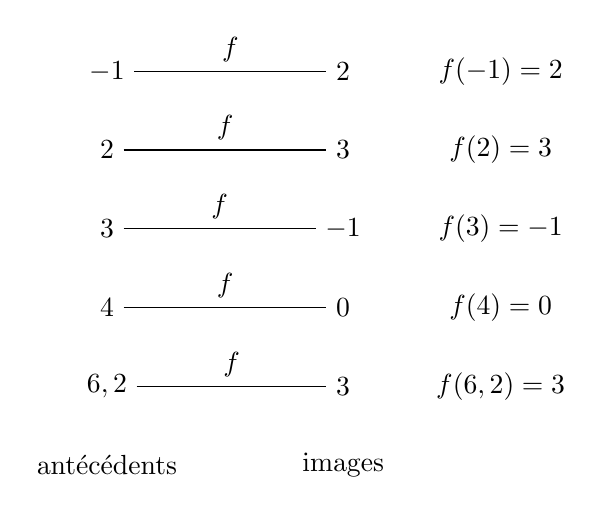
\begin{tikzpicture}
			\coordinate (X) at (0,0);
			\coordinate (Y) at (3,0);
			\foreach \x/\y in {-1/2,2/3,3/-1,4/0,{6,2}/3} {
					\node (X) at ($(X) + (0,-1)$) {$\x$};
					\node (Y) at ($(Y) + (0,-1)$) {$\y$};
					\path[\myArrow] (X) edge node[above] {$f$} (Y);
					\node at ($(Y) + (2,0)$) {$f(\x) = \y$};
				}

			\node at ($(X) + (0,-1)$) {antécédents};
			\node at ($(Y) + (0,-1)$) {images};
		\end{tikzpicture}
	\end{center}
\end{frame}

\begin{frame}
	$f(x)$ est \textbf{L'image} de $x$ par la fonction $f$. On représente une image par la lettre $y$, et on écrit alors

	$$ f(x) = y $$

	Dans ce cas, $x$ est \textbf{UN antécédent} de $y$.

	\pause

	\begin{tcolorbox}
		\begin{itemize}
			\item Il n'y a \uline{qu'une seule image} pour un nombre donné.
			\item Il peut y avoir \uline{plusieurs antécédents} pour un nombre donné.
		\end{itemize}
	\end{tcolorbox}
\end{frame}

\begin{frame}
	Deux principales manières de représenter une fonction : \bigskip

	\begin{minipage}{0.47\textwidth}
		\begin{center}
			Algébriquement :

			$$ f(x) = \dfrac{1}{2}x - 1 $$
		\end{center}
	\end{minipage}
	\begin{minipage}{0.47\textwidth}
		\begin{center}
			Graphiquement :

			\begin{tikzpicture}[scale=0.7]
				\tikzRepere{-3}{3}{-3}{3}
				\draw[very thick,red,domain=-3:3] plot({\x},{0.5*\x - 1}) node[right] {$𝒞_f$};
			\end{tikzpicture}
		\end{center}
	\end{minipage}
\end{frame}

\end{document}